


\chapter{pure yap}
\begin{itemize}
    \item Relationship between explanatory- and response variables is not required to be linear.
    \item Inclusion of random effects in non-linear framework results in the absence of a closed form expression for the likelihood function - this implies we have to use methods to approximate the likelihood function
    \item Approximation methods
    \item HOW TO BUILD POP-PK-MODEL: See Bonate p. 263 - modelbygningen opdeles i fem steps (har forkortet dem ned her):
    \begin{enumerate}
        \item Determine the structual PK model (ligesom vi gør i preliminary) and estimate the model without covariates
        \item Examine the assumptions regarding the distribution of random effects
        \item Select covariates for inclusion in the model (covariate screening)
        \item Build the model using covariates (redundant if the covariates were tested directly in the NLME model)
        \item Evaluate final parameter estimates - test assumptions to validate the model
    \end{enumerate}
\end{itemize}
We want to allow for individual variability for the PK parameters. An an example we might want to model the elimination rate as
\begin{align*}
    K_{e,i}=K_{e,pop}\left(\frac{\text{covariate}_i}{\text{ covariate}_{pop}}\right)^{\alpha}\exp({\eta_{K_{e,i}}}), 
\end{align*}
where $K_{e,i}$ is the elimination rate for subject $i$, $K_{e,pop}$ is the population mean for $K_{e}$, $\eta_{K_{e,i}} \sim N(0, \omega^2)$ is the subject variability, and $\alpha$ is a constant indicating the influence of the covariate.


% \section{Modelopbygning}
% \begin{align*}
%     y_i &= (y_{1,i},\dots,y_{1,n_i})^\top \in \R^{n_i}\\
%     Y&=(y_1,y_2,\dots,y_N)^\top= (y_{1,1},\dots,y_{1,n_1},y_{2,1},\dots,y_{2,n_2},\dots,y_{N,1},\dots,y_{N,n_N})^\top \in \R^{n_1+n_2+\cdots+n_N}\\
%     g(t,u,\theta)&=(g_1(\theta_1),g_2(\theta_2),\dots,g_N(\theta_N))^\top \in \R^{n_1+n_2+\cdots+n_N}\\
%     \epsilon &= (e_1,e_2,\dots,e_N)^\top=(e_{1,1},\dots,e_{1,n_1},e_{2,1},\dots,e_{2,n_2},\dots,e_{N,1},\dots,e_{N,n_N})^\top \in \R^{n_1+n_2+\cdots+n_N}\\
%     Y &= G(t,u,\theta) + \epsilon\\
%     \theta &= [(h(a_1,\beta,\eta_1),h(a_2,\beta, \eta_2), \dots,h(a_N,\beta,\eta_N)]^\top \in \R^{pN}\\
%     e_{i,j} &\sim (0,\sigma^2)\\
%     e_i &\sim (0,R_i), R_i \in \R^{n_i \times n_i}\\
%     \eta_i &\sim (0,\Omega), \Omega \in \R^{r \times r}\\
%     \eta &= (\eta_{1,1},\eta_{1,2},\dots,\eta_{1,N},\dots,\eta_{r,1},\dots,\eta_{r,N})=  (\eta_1,\dots,\eta_N)^\top \in \R^{rN}\\
%     \eta &\sim (0,\Sigma)\\
%     \Sigma &=
% \begin{bmatrix}
%     \Omega & O & \cdots & O \\
%     O & \Omega & \cdots & O \\
%     \vdots & \vdots & \ddots & \vdots \\
%     O & O & \cdots &\Omega
% \end{bmatrix}
%  \in \R^{rN \times rN}\\
%      R &=
% \begin{bmatrix}
%     R_1 & O & \cdots & O \\
%     O & R_2 & \cdots & O \\
%     \vdots & \vdots & \ddots & \vdots \\
%     O & O & \cdots & R_N
% \end{bmatrix}
%  \in \R^{(n_1+n_2+\dots+n_N)\times (n_1+n_2+\dots+n_N)}\\
%  \Omega &= \begin{bmatrix}
%     \omega_{1,1} & \omega_{1,2} & \cdots & \omega_{1,r} \\
%     \omega_{2,1} & \omega_{2,2} & \cdots & \omega_{2,r} \\
%     \vdots & \vdots & \ddots & \vdots \\
%     \omega_{r,1} & \omega_{r,2} & \cdots & \omega_{r,r}
% \end{bmatrix}, \quad \omega_{k,m} = \Cov{\eta_{i,k},\eta_{i,m}}.
% \end{align*}

% % \section{Residual variance models}
% % %Bonat side 243
% % The variability that remains unexplained by a NLME-model is referred to as the residual variance. This residual variance is explicitly represented as the error term in the first stage of an NLME-model, represented in \eqref{eq: NLME Stage 1}, and can be modeled with a residual variance model. As the residual variance becomes larger or more heterogeneous, it becomes increasingly more important to include a residual variance model to the overall model. In \eqref{eq: NLME Stage 1}, the error term is added to the non-linear function, and therefore, the residual variance model used, is the additive residual variance model. This is the most commonly used model, but is not always valid. Incorporating a residual variance model that is not suitable to the data can lead to inaccurate results. For instance, consider modeling the drug concentration of a patient who received a single dose administered EV. If an additive residual variance model is used, where the error term, $e_{i,j}$, follows a normal distribution with mean $0$ and variance $\sigma^2$, the model can theoretically yield negative concentration values, for a large time, and if the error term is sufficiently large and negative, see Figure \ref{fig: Residual variance model add}. However, since negative concentrations are practically impossible, this model is inappropriate to use. Instead, in this case, a model that restricts the concentration values to non-negative values should be employed.

% % The first stage of the NLME-model \eqref{eq: NLME Stage 1} can be extended, such that it includes the structural form and the parameters associated with the residual variance model. This extension is
% % \begin{align} \label{eq: residual variance model}
% %     y_{i,j} &= g(t_{i,j}, u_i, \theta_i) + v(\Phi, t_{i,j}, u_i, \theta_i)e_{i,j},
% % \end{align}
% % where $v(\cdot)$ denotes the variance function and $\Phi$ denotes the parameters of the residual variance model. Given that $v(\cdot)$ is constant and $e_{i,j}$ is considered to be independent from $g(t_{i,j}, u_i, \theta_i)$, have mean zero, and variance $\sigma^2$, the variance for the extended model is
% % \begin{align*}
% %     \Var{y_{i,j}} = \sigma^2 [v(\Phi, t_{i,j}, u_i, \theta_i)]^2 .
% % \end{align*}
% % The most common residual variance models are seen in Table \ref{tab:error models}. Across all models, it is assumed that the residuals, $e_{i,j}$ has mean zero, constant variance $\sigma^2$, and are independent of the non-linear function $g(t_{i,j}, u_i, \theta_i)$.
% % \begin{table}[H]
% % \centering
% % \begin{tabular}{>{\raggedright\arraybackslash}p{0.4\textwidth}>{\raggedright\arraybackslash}p{0.5\textwidth}}
% % \toprule
% % \textbf{Residual Variance Model} & \textbf{Representation} \\
% % \midrule
% % Additive error & $y_{i,j} = g(t_{i,j}, u_i, \theta_i) + e_{i,j}$ \\
% % Proportional error & $y_{i,j} = g(t_{i,j}, u_i, \theta_i)(1+e_{i,j})$ \\
% % Combined additive and proportional error & $y_{i,j} = g(t_{i,j}, u_i, \theta_i) + \left( \sqrt{1-\phi_k + \phi_k g(t_{i,j}, u_i, \theta_i)^2}\right)e_{i,j}$, \quad $\phi_k \in [0, 1]$ \\
% % \bottomrule
% % \end{tabular}
% % \caption{Residual variance models and their respective representation.}
% % \label{tab:error models}
% % \end{table}
% % The residual variance models presented in Table \ref{tab:error models} exhibit different properties, with the first model, being the additive residual variance model. It is characterized by the error term being added to the non-linear function. As the variance of the error is constant, and the error term is independent of the non-linear function, $g(t_{i,j}, u_i, \theta_i)$, the variance of the model is constant over time,
% % \begin{align*}
% %     \Var{y_{i,j}} = \Var{g(t_{i,j}, u_i, \theta_i) + e_{i,j}} = \sigma^2.
% % \end{align*}
% % An example of simulated data that follows the additive residual variance model can be seen in Figure \ref{fig: Residual variance model add}.

% % The second model in Table \ref{tab:error models} is the proportional residual variance model. In this model the error term is multiplied with the non-linear function, resulting in the model
% % \begin{align*}
% %    y_{i,j}=g(t_{i,j}, u_i, \theta_i) + g(t_{i,j}, u_i, \theta_i)e_{i,j},
% % \end{align*}
% % where $g(t_{i,j}, u_i, \theta_i)$ is multiplied with the error, and therefore represents the residual variance function $v(\cdot)$ from \eqref{eq: residual variance model}. As the variance of the error term is constant but proportional with the non-linear function, the variance of the model is proportional with the non-linear function,
% % \begin{align*}
% %     \Var{y_{i,j}} = \Var{g(t_{i,j}, u_i, \theta_i) + g(t_{i,j}, u_i, \theta_i)e_{i,j}} = \sigma^2 \left[g(t_{i,j}, u_i, \theta_i) \right]^2.
% % \end{align*}
% % The proportional residual variance model can be seen in Figure \ref{fig: Residual variance model prop}.

% % The third model in Table \ref{tab:error models} is a combination of the additive and proportional error models, which means it exhibits properties from both models. As $\phi_k \in [0,1]$, it is possible to adjust the contribution of each model. Note that if $\phi_k=0$, the residual variance model simplifies to an additive model, whereas if $\phi_k=1$, it corresponds to a proportional model. The variance of the model is
% % \begin{align*}
% %     \Var{y_{i,j}} &= \Var{g(t_{i,j}, u_i, \theta_i) + \left( \sqrt{1-\phi_k + \phi_k g(t_{i,j}, u_i, \theta_i)^2}\right)e_{i,j}} \\
% %     &= \sigma^2 \left[1-\phi_k + \phi_k g(t_{i,j}, u_i, \theta_i)^2\right].
% % \end{align*}
% % The combined additive and proportional residual variance model can be seen in Figure \ref{fig: Residual variance model add prop}.

% % \begin{figure}[H]
% %     \centering
% %     \begin{minipage}{0.45\textwidth}
% %         \centering
% %         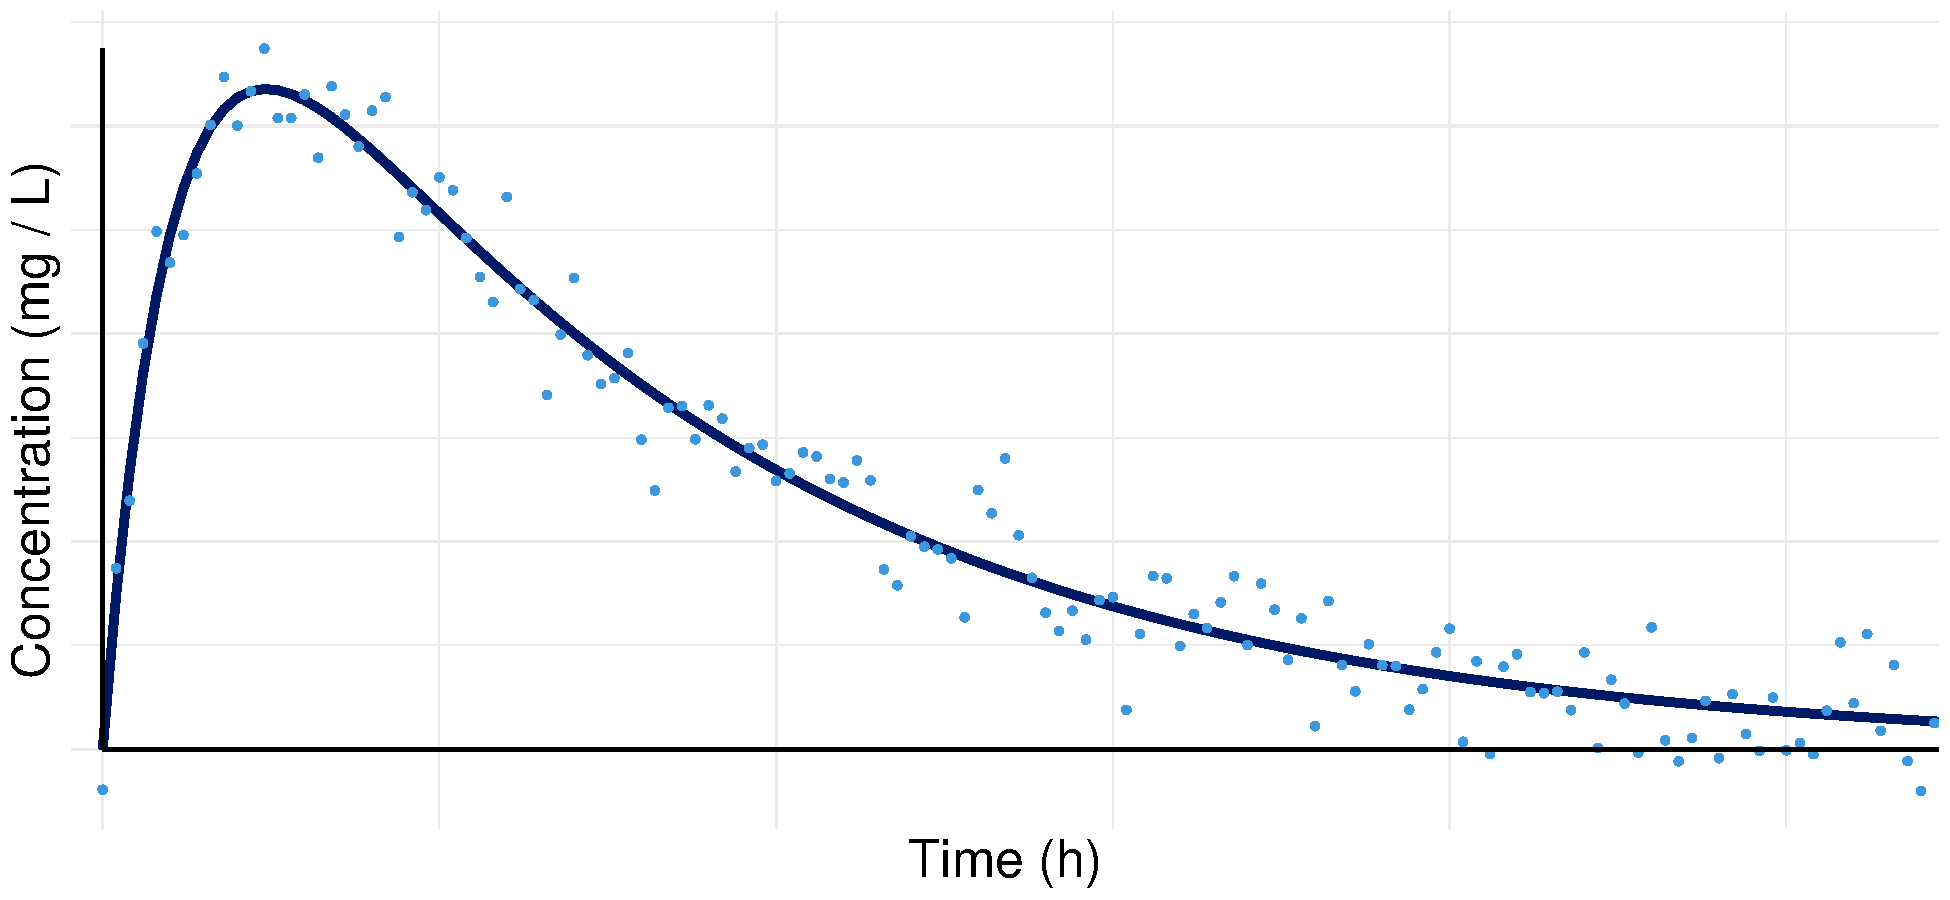
\includegraphics[width=\linewidth]{fig/img/Residual Variance Model/Concentration W. Oral Add.pdf}
% %         \caption{Additive error}
% %         \label{fig: Residual variance model add}
% %     \end{minipage}%
% %     \hfill
% %     \begin{minipage}{0.45\textwidth}
% %         \centering
% %         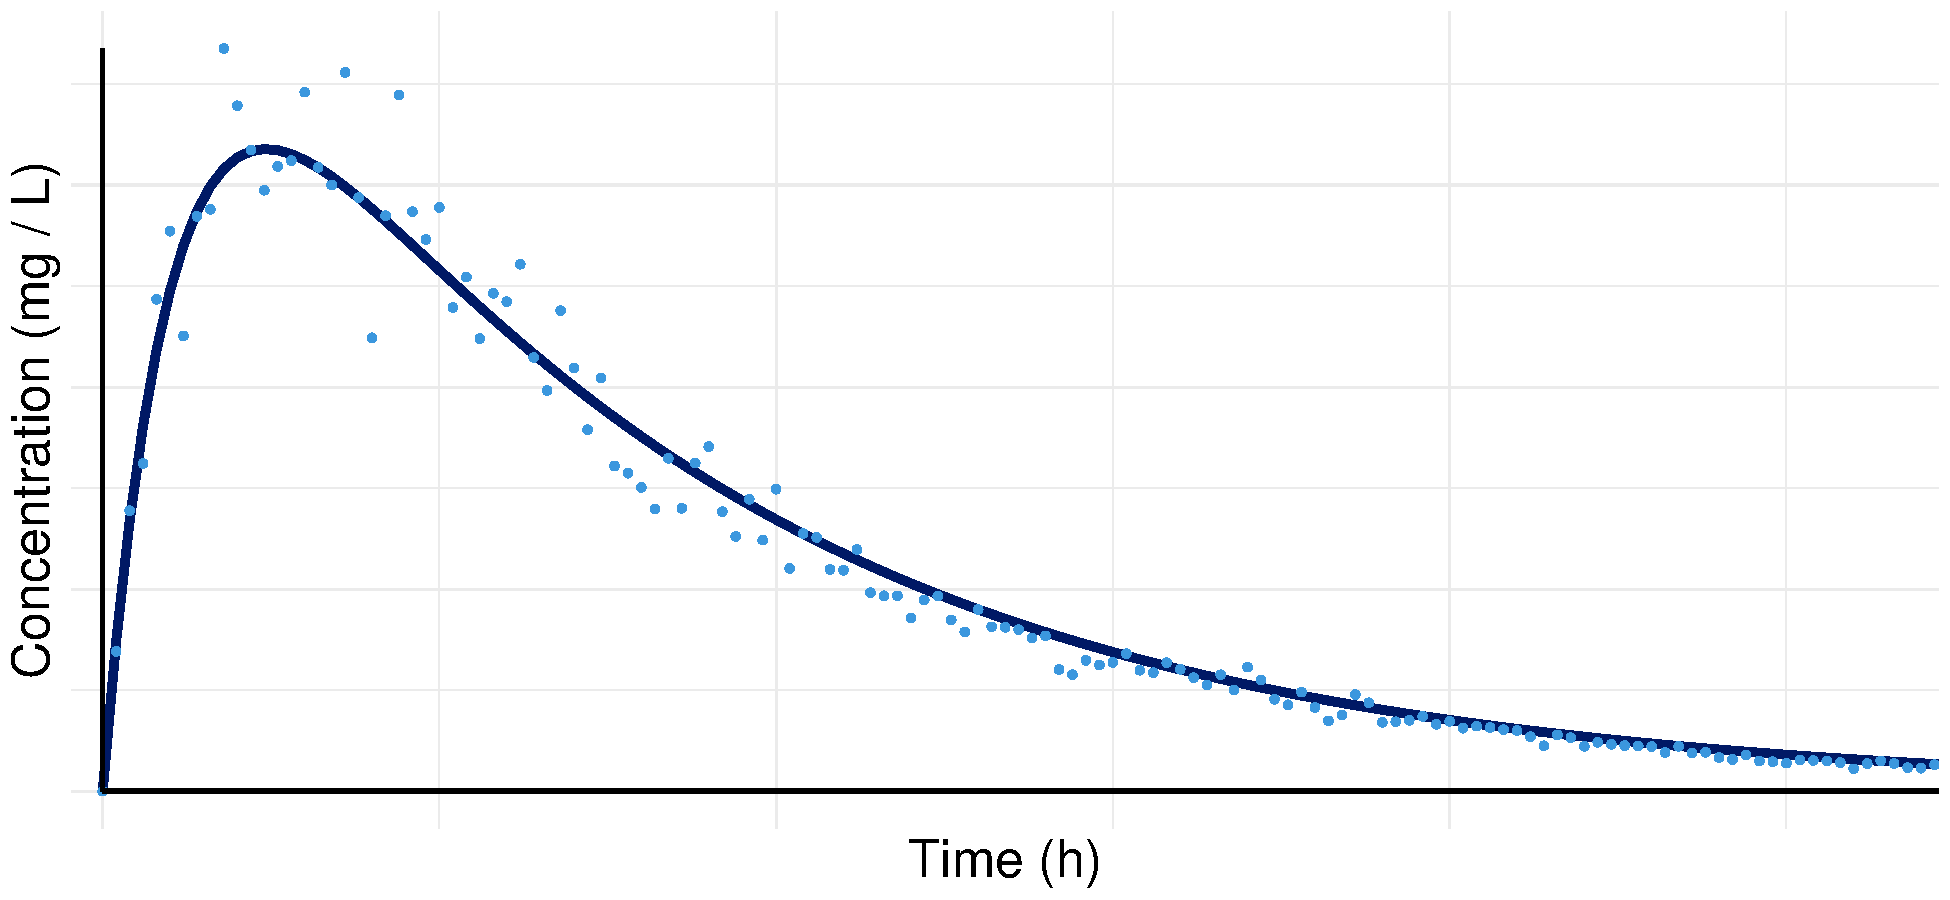
\includegraphics[width=\linewidth]{fig/img/Residual Variance Model/Concentration W. Oral Prop.pdf}
% %         \caption{Proportional error}
% %         \label{fig: Residual variance model prop}
% %     \end{minipage}
% %     \vfill

% %     \begin{minipage}{0.45\textwidth}
% %         \centering
% %         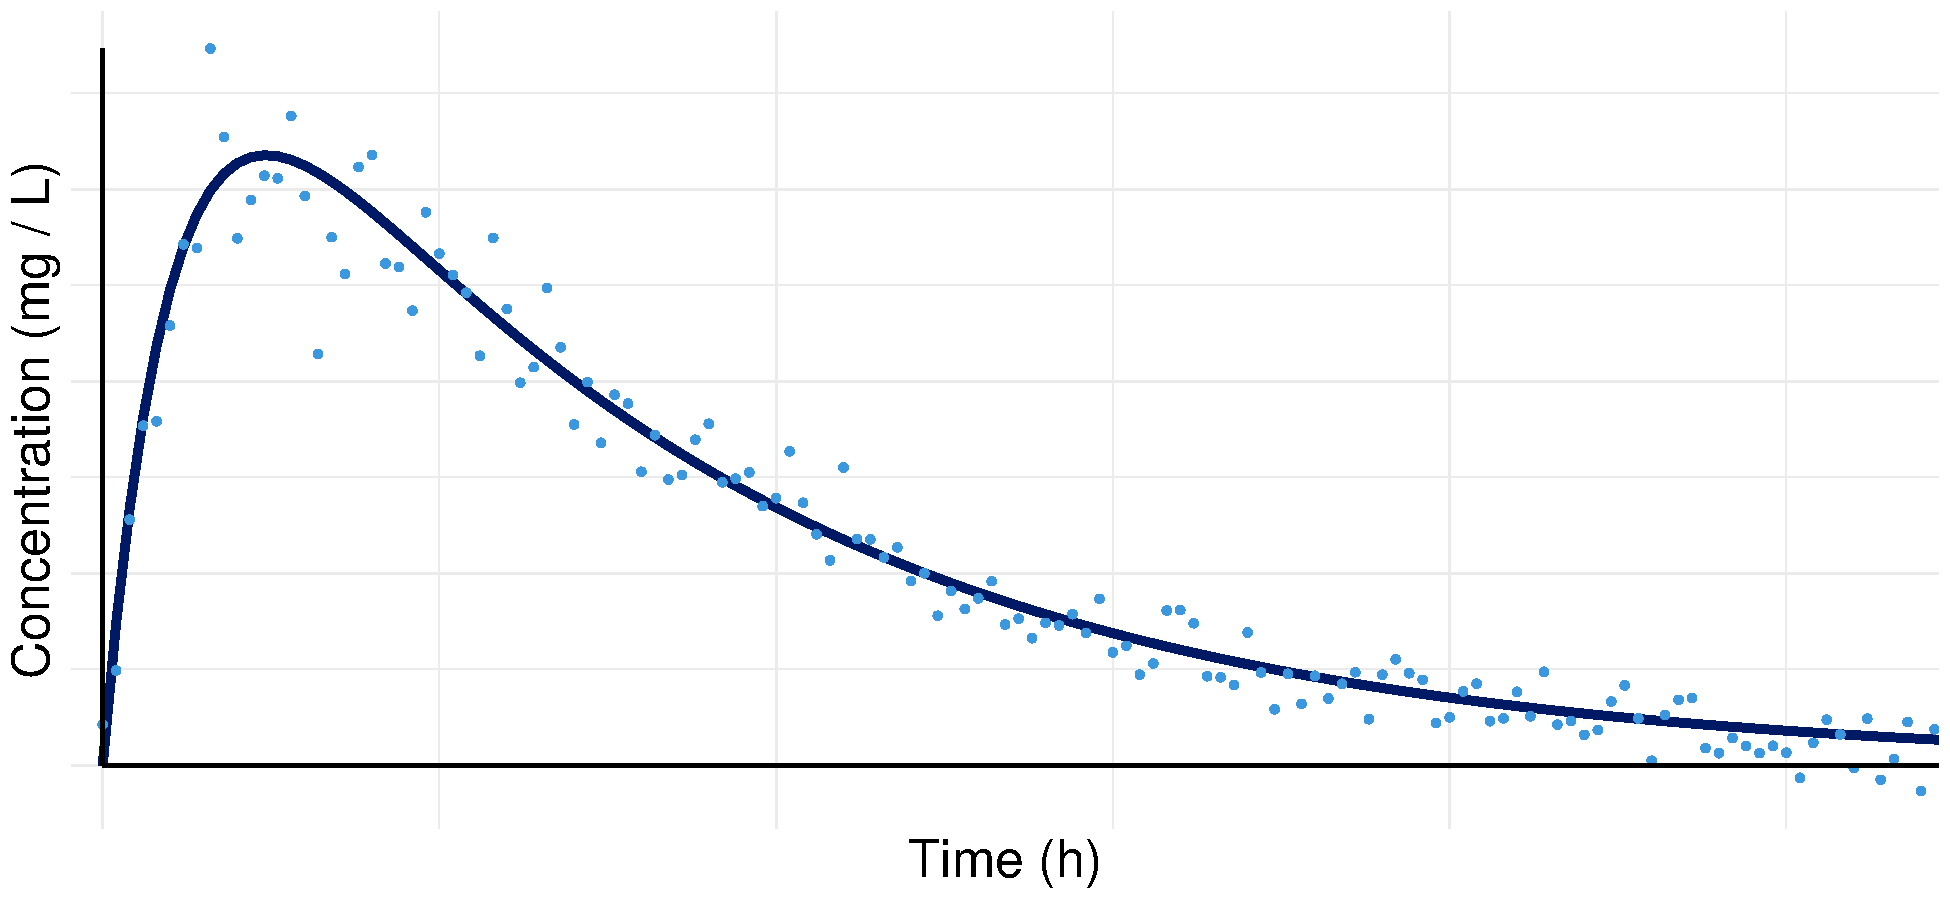
\includegraphics[width=\linewidth]{fig/img/Residual Variance Model/Concentration W. Oral Add Prop.pdf}
% %         \caption{Combined additive and proportional error}
% %         \label{fig: Residual variance model add prop}
% %     \end{minipage}
% %     \caption{Simulated concentrations from a single dose one-compartment model with EV administration, each with different residual variance structures.}
% %     \label{fig: Residual variance model}
% % \end{figure}
% % To determine which residual variance model is most suitable, likelihood ratio tests and goodness of fit plots of each model are evaluated. \\